\newpage
% !TeX spellcheck = it_IT
\section{Memory Hierarchy}
I principi fondamentali che andremo a vedere sono legati alle tecnologie con cui vengono costruite le memorie, la gerarchia delle varie tipologie di memorie, le memorie caches ed in fine come andare a misurare e migliorare le performance delle caches.

\subsection{Memory technologies}
Partiamo dicendo che esistono varie tipologie di memorie, che possono essere distinte in primo luogo in \textbf{memorie volatili}, e \textbf{memorie non volatili}. Quelle volatili sono:
\begin{wrapfigure}{r}{5cm}
	\centering
	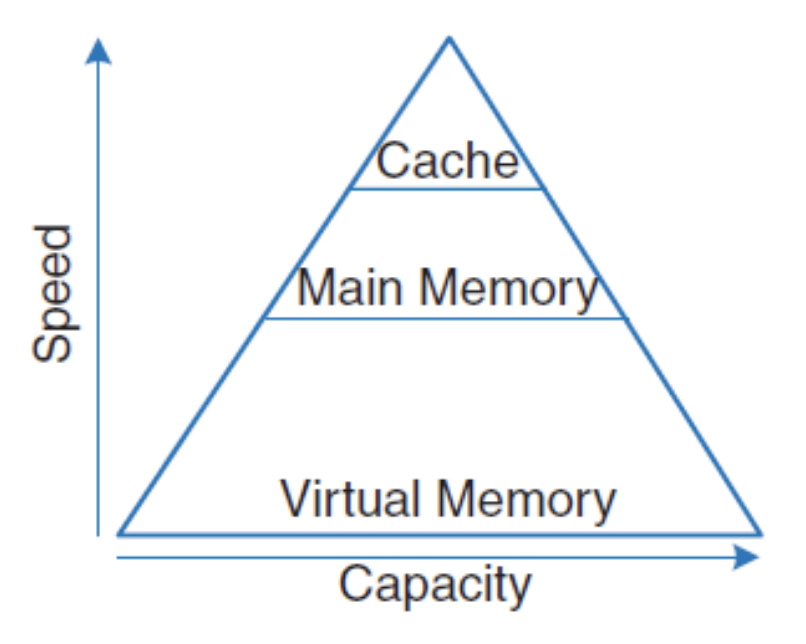
\includegraphics[width=4cm]{images/memory-hierarcgy.png}
	\caption{Gerarchia memoria}
\end{wrapfigure}

\begin{itemize}
    \item Latches, flip-flops, register files (o semplici registri).
    \item SRAM (Static Random-Access Memory).
    \item DRAM (Dynamic Random-Access Memory).
\end{itemize}

\noindent Fra le memorie non volatili invece ci sono:
\begin{itemize}
    \item ROM
    \item NVRAM \footnote{Memoria non volatile nel formato di un banco DRAM che può fornire accesso tramite byte-address.}
    \item Flash memory
    \item Magnetic disks
\end{itemize}

\subsection{Cost vs Capacity vs Access Time}
Un altro confronto interessante da fare fra le memorie è relativamente ai costi, le capacità ed il tempo di accesso.
\begin{center}
	\begin{tabular}{|c|c|c|c|c|}
	\hline
	\textbf{Memoria} &\textbf{Access time (ns)} & Bandwidth (GB/s) & \textbf{Price(\$/GB)} & \textbf{Usage} \\
	\hline
	\textit{SRAM} & $0.5-1$ & $25+$ & $5000$ & Register and caches \\
	\hline
	\textit{DRAM} & $10-50$ & $10$ & $7$ & RAM \\
	\hline
	\textit{Flash} & $20.000$ & $0.5$ & $0.40$ & SSD disks \\
	\hline
	\textit{Magnetic} & $5.000.000$ & $0.75$ & $0.05$ & HDD Disk \\
	\hline
\end{tabular}
\end{center}

\hspace{-15pt}Da questa classificazione possiamo trarre alcune regole generali:
\begin{itemize}
    \item Le memorie di grandi dimensioni sono solitamente lente e economiche.
    \item Le memorie di piccole dimensioni sono più veloci ma anche più costose.
\end{itemize}

\noindent Da qui possiamo capire che nella selezione della memorie va trovato un compromesso fra i parametri visti precedentemente per andare ad avere memorie sufficientemente grandi per contenere i dati richiesti ma allo steso tempo sufficientemente veloci per evitare il \textbf{von Neumann Bottleneck}.

\newpage
\subsection{Von Neumann architecture}
\begin{wrapfigure}{r}{6.5cm}
    \vspace{-25pt}
    \centering
    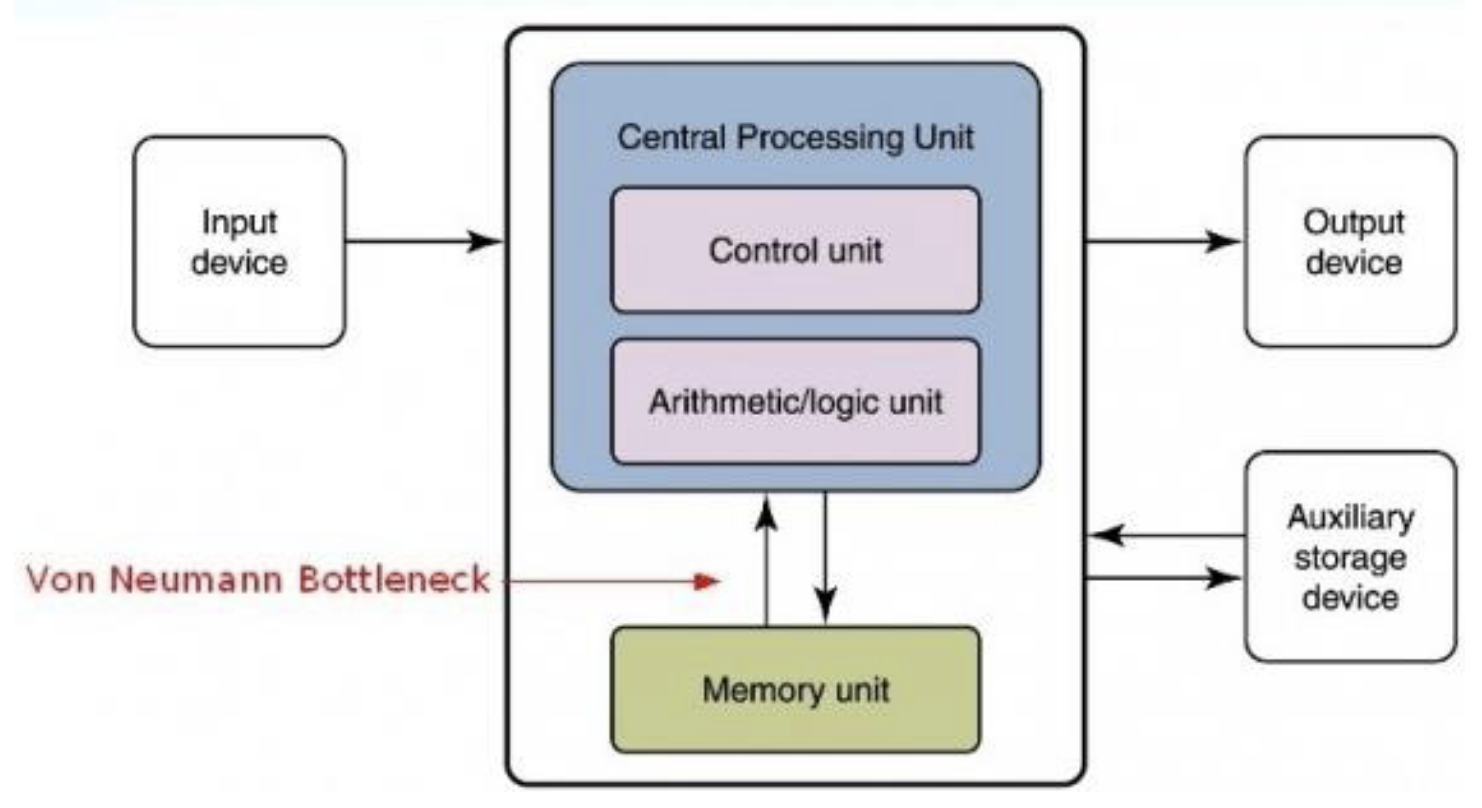
\includegraphics[width=6cm]{images/von-numan.png}
    \caption{Von-Neumann}
\end{wrapfigure}
Le performance dei computer sono limitate nella velocità della CPU dal trasferimento di dati fra le memorie esterne dall'unità di calcolo.\\
Per mitigare questo problema inseriamo memorie più piccole e veloci vicino al processore, mentre più ci si allontana più si avranno memorie grosse e lente. In questo modo facciamo lavorare il processore alla velocità della memoria più vicina.\\\\

\begin{wrapfigure}{l}{6.5cm}
    \vspace{-10pt}
    \centering
    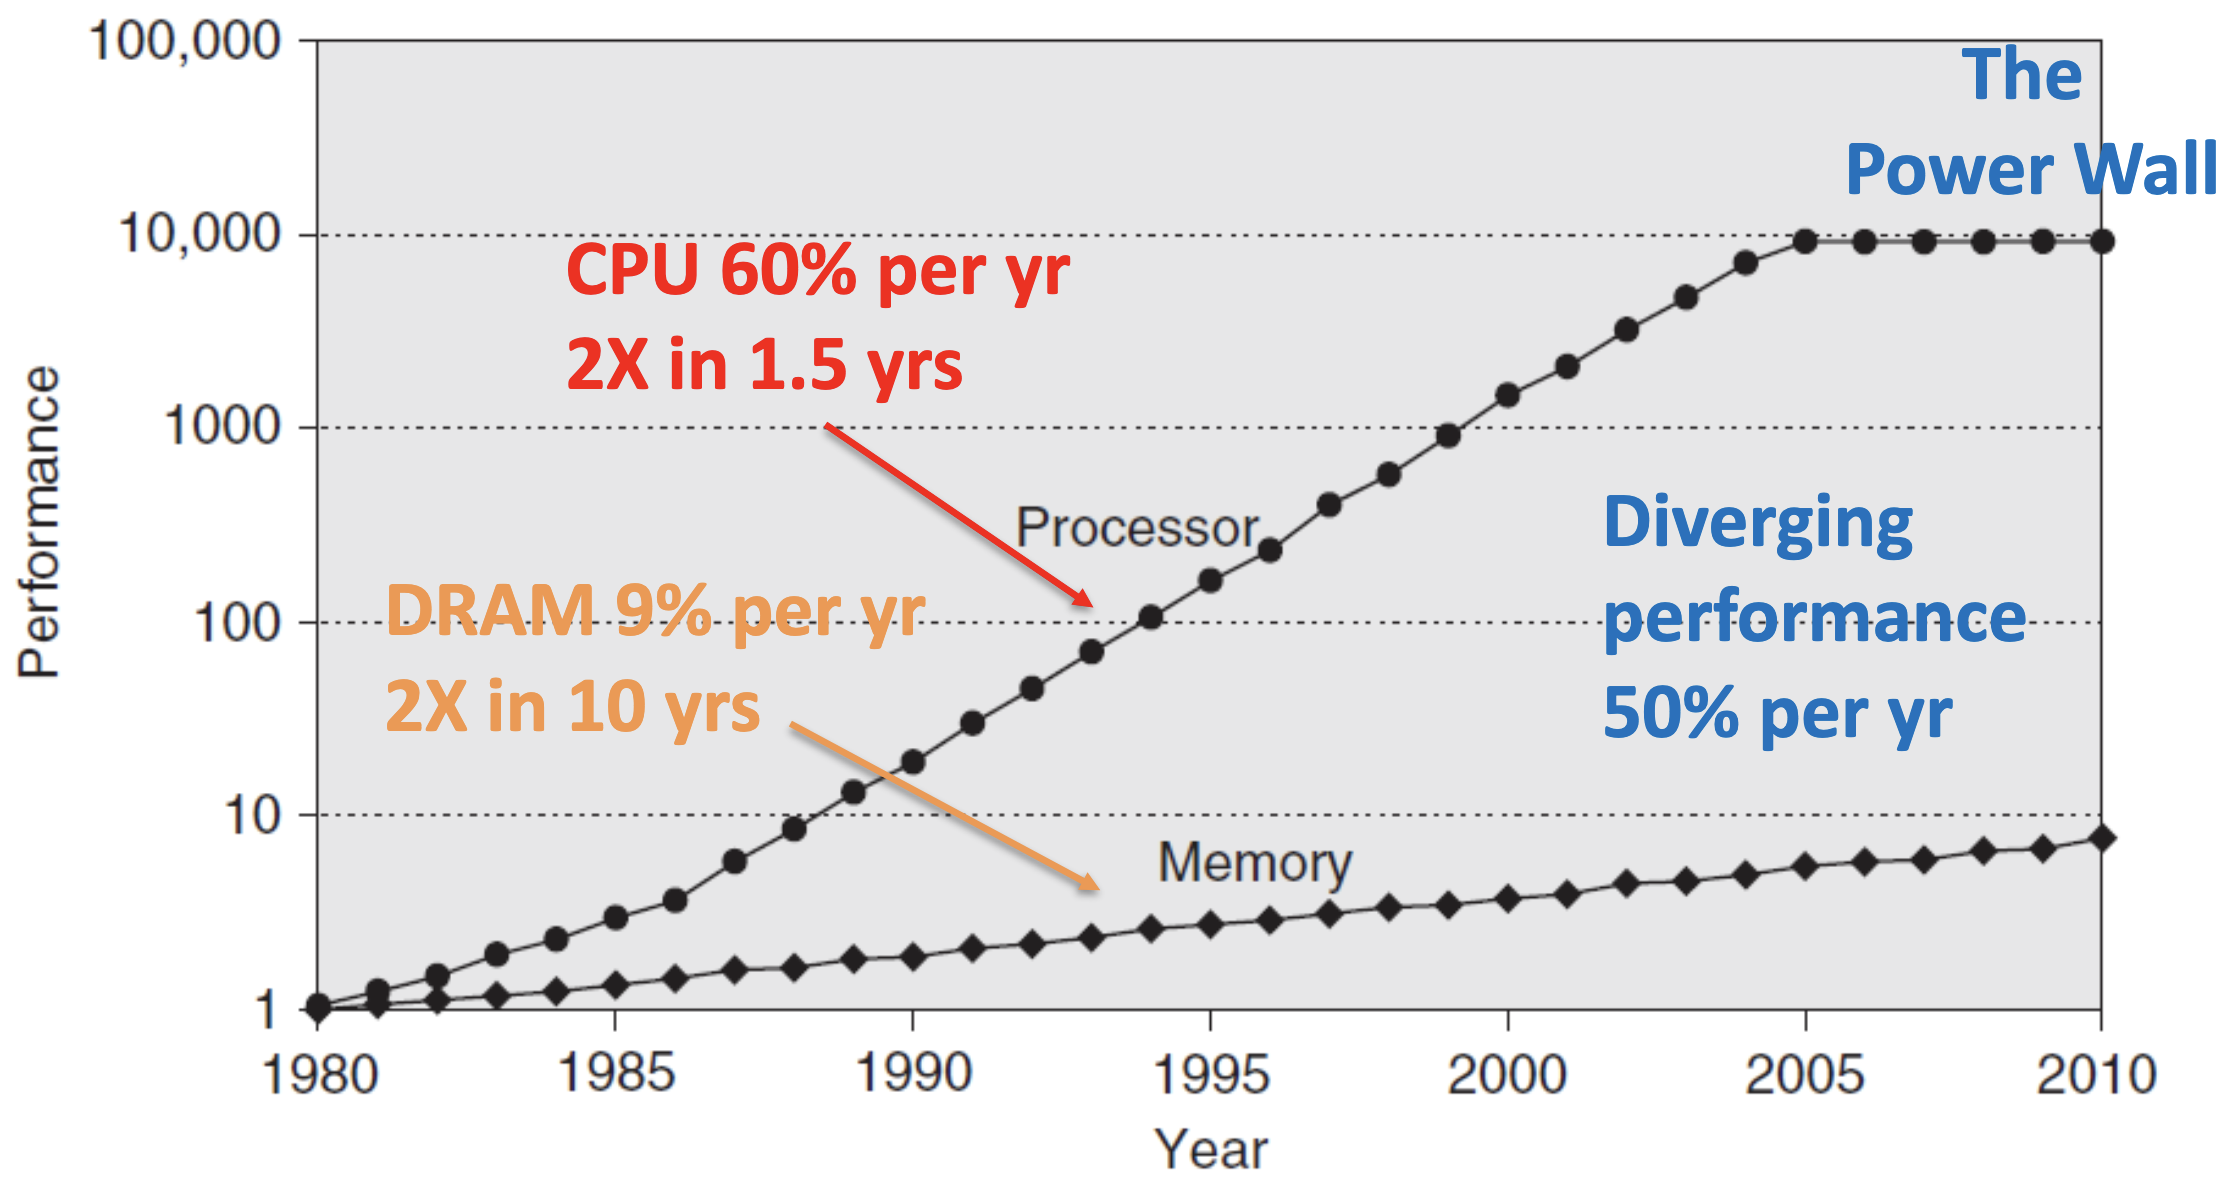
\includegraphics[width=6cm]{images/von-newmann-bottleneck.png}
    \caption{Von-Neumann Bottleneck}
\end{wrapfigure}
L'obiettivo è quindi di fornire l'\textbf{illusione} di avere una memoria grande quanto la memoria più lontana e veloce quanto la memoria più vicina.
Per farlo facciamo risiedere i dati inizialmente nel livello più lontano e più capiente. Per far accedere il processore bisognerà spostare i dati tra i vari livelli di gerarchia.\\
Questo metodo presenta alcune problematiche: serve un meccanismo che, se un dato è già presente un certo livello, determini quello giusto e un meccanismo che permetta di rimpiazzare certi dati per poter fare spazio.\\


\subsection{Terminologia}
Introduciamo ora un po' di terminologia che ci servirà successivamente.

\begin{definition}[Hit e Miss]
Se i dati richiesti dal processore compaiono in qualche blocco nel livello di memoria più vicino, si parla di \textbf{hit}. In caso contrario, si parla di \textbf{miss} e si accede al livello di memoria successivo per recuperare il blocco contenente i dati richiesti.
\end{definition}

\begin{definition}[Hit rate]
    L'hit rate (frequenza di successi) è la frazione di accessi alla memoria rilevati nel livello superiore (ovvero, più vicino alla CPU), utilizzata come misura delle prestazioni della gerarchia.
\end{definition}

\begin{definition}[Miss rate]
    Il miss rate è la frazione di accessi alla memoria non trovati nel livello superiore.
\end{definition}

\begin{definition}[Miss penalty]
    La miss penalty è il tempo necessario per sostituire un blocco nel livello $n$ con il blocco corrispondente dal livello $n-1$.
\end{definition}

\begin{definition}[Miss time]
    Il miss time è il tempo per ottenere l'elemento in caso di tempo di miss. 
    \begin{equation*}
    	\text{miss time} = \text{miss penalty} + \text{hit time}
    \end{equation*}
\end{definition}

\noindent Il \textbf{miss rate} e l'\textbf{hit rate} si calcolano con le seguenti formule:
\begin{equation}
    MR = \frac{\text{Number of misses}}{\text{Number of total memory access}} = 1 - HR
\end{equation}
\begin{equation}
    MR = \frac{\text{Number of hits}}{\text{Number of total memory access}} = 1 - MR
\end{equation}

\subsubsection{AMAT}
Definiamo l'Average Memory Access Time:
\begin{equation}
    AMAT = t_{M0} + MR_{M0} * (t_{M1} + MR_{M1} * (t_{M2} + MR_{M2} * (t_{M3} + \ldots)))
\end{equation}
$t_{M0}$ = hit time, $MR_{M0}$ = miss rate, $(t_{M1} + MR_{M1} * (t_{M2} + MR_{M2} * (t_{M3} + \ldots))$ = miss penalty.

\begin{observation}
Se l'hit rate è abbastanza alto, la gerarchia della memoria ha un tempo di accesso effettivo vicino a quello del livello più alto (e più veloce) e una dimensione uguale a quella del livello più basso (e più grande).
\end{observation}

\begin{example}
	Consideriamo una memoria con una gerarchia su 3 livelli con i seguenti valori:
	\begin{center}
		\begin{tabular}{|c|c|c|}
			\hline
			\textbf{Livello} & \textbf{Miss rate} & \textbf{Hit time} \\
			\hline
			L1 & 5\% & $t_{L1}$ \\
			L2 & 2\% & $t_{L2}$ \\
			L3 & 100\% & $t_{L3}$ \\
			\hline
		\end{tabular}
	\end{center}
	Quindi il valore AMAT sarà:
	\begin{equation*}
		AMAT= t_{L1} + 0.05 * (t_{L2} + 0.02 * t_{L3}) = t_{L1} + 0.05 * t_{L2} + 0.001 * t_{L3}
	\end{equation*}
\end{example}

\subsection{The locality principle}
Il principio di località di riferimento (o locality principle) si riferisce al fenomeno per il quale un programma tende ad accedere alla stessa locazione di memoria per un determinato periodo.\\
Possiamo osservare che, se il programma fa riferimento ad una locazione di memoria allora:
\begin{itemize}
	\item la stessa locazione di memoria verrà riutilizzerà a breve con alta probabilità
	\item gli elementi "vicini" alla posizione di memoria appena raggiunta saranno presto referenziati con un'alta probabilità
\end{itemize}

Il principio di località è la forza trainante che rende la gerarchia della memoria funzionante. Esso infatti incrementa la probabilità di riutilizzare dei blocchi di dati che erano stati precedente mossi da un livello $n$ ad un livello $n-1$, riducendo il miss rate.\\ Il programmatore dovrà comunque fare attenzione ad implementare questo principio.

\subsubsection{Locality characterization}
Andiamo a distinguere due tipologie di località. 
\begin{itemize}
    \item \textbf{La località temporale} (o riuso di dati): i dati riferiti precedentemente probabilmente verranno riferiti nuovamente in un breve lasso di tempo.
    \begin{example}[Località temporale]
    Consideriamo il seguente codice:
    \begin{lstlisting}
    	for(int i=0; i<10; i++)
    		s1 += i; s2 -= 1;
    \end{lstlisting}
    In questo caso le locazioni di memoria che contengono s1 ed s2 hanno località temporale.
    \end{example}
    Dunque se all'interno della gerarchia della memoria teniamo i dati più recenti, secondo il principio di località ci riaccederò nuovamente dopo poco tempo.
    
    \item \textbf{Località spaziale}: dati vicini a quelli a cui sto facendo riferimento saranno probabilmente utilizzati a breve.
    \begin{example}[Località spaziale]
    	Consideriamo il seguente codice:
    	\begin{lstlisting}
    		for(int i=0; i<10; i++)
    			func(A[i]);
    	\end{lstlisting}
    	In questo caso le locazioni di memoria dell'array hanno località spaziale, visto che sono implementate in modo contiguo.
    \end{example}
    Dunque se all'interno della gerarchia della memoria teniamo i dati vicini a quelli in utilizzo, secondo il principio di località ci saranno grosse probabilità di accedervi con la CPU.
\end{itemize}


\subsection{Traferimiento dati}
I dati si trasferiscono solamente attraverso due memorie adiacenti. Per ottimizzare il caricamento dei dati esso viene fatto come \textbf{blocchi} di dimensione granulare (parole) in modo da poter sfruttare la località spaziale. La dimensione dei blocchi può cambiare attraverso i livelli.\\
Per la cache i blocchi vengono chiamati \textit{cache line} o \textit{cache block} (tipicamente 64-128 bytes, 8-16 parole). Per le RAM invece abbiamo \textit{pagine di segmenti}, mentre per i dischi abbiamo \textit{blocchi di dischi}.\\

\noindent Consideriamo il seguente codice in C e il suo corrispettivo in assembly.
\begin{figure}[!h]
\begin{minipage}[t]{0.45\linewidth}
\centering
\begin{lstlisting}
// Sum and A are global variables
int i;
for(int i=0; sum=0; i<N, i++){
    sum += A[i];
}
\end{lstlisting}
\end{minipage}
\hspace{.35cm}
\begin{minipage}[t]{0.45\linewidth}
\begin{lstlisting}[language={[x86masm]Assembler}]
@ r0=&A, r1=&sum, r2=N, r3=i
loop: cmp r3, r3
      beq end
      ldr r12, [r0, r3, lsl #2]
      ldr r4, [r1]
      add r4, r4, r12
      str r4, [r1]
      add r3, r3, #1
      b loop
end: ...
\end{lstlisting}
\end{minipage}
\end{figure}

In questo frammento di codice il loop viene eseguito N volte, e quindi ogni struttura viene richiesta N volte in maniera sequenziale. In questo caso sia la localizzazione temporale che spaziale viene utilizzata.\\
'Sum' è ripetutamente letta e scritta, quindi utilizza la località temporale, 'A' è salvata come un insieme contiguo di celle di memoria, quindi utilizza la località spaziale.